\documentclass[UTF8]{ctexart}
\usepackage{picinpar, graphicx} % 导入这个库后,就能支持插入表格
\usepackage{algorithm, algorithmic} % 支持数学公式输入

\title{你的标题写在这里}
\author{作者名字}
\date{\today}

\begin{document}
	\maketitle  %这行代码, 让你前面的 title, author, date生效
	\newpage  %分页
	
	\section{大标题} %大标题
	中文论文排版测试。
	\subsection {第二级标题} %会形如: 1.1,  2.1,   3.1 
	\subsubsection {第三级标题} %会形如 1.1.1,   2.1.1
	
	%插入表格
	\begin{table}[!t]
		\renewcommand{\arraystretch}{1.3}
		\caption{An Example of a Table}
		\label{table_example}
		\centering
		\begin{tabular}{|c||c|}
			\hline
			One & Two\\
			\hline
			Three & Four\\
			\hline
		\end{tabular}
	\end{table}


%插入图片. 图片目录一定要和.tex文件在同一目录下.
% 另外注意: [!t]、[width=2.5in] 这个是不能缺的
\begin{figure}[!t]
	\centering
	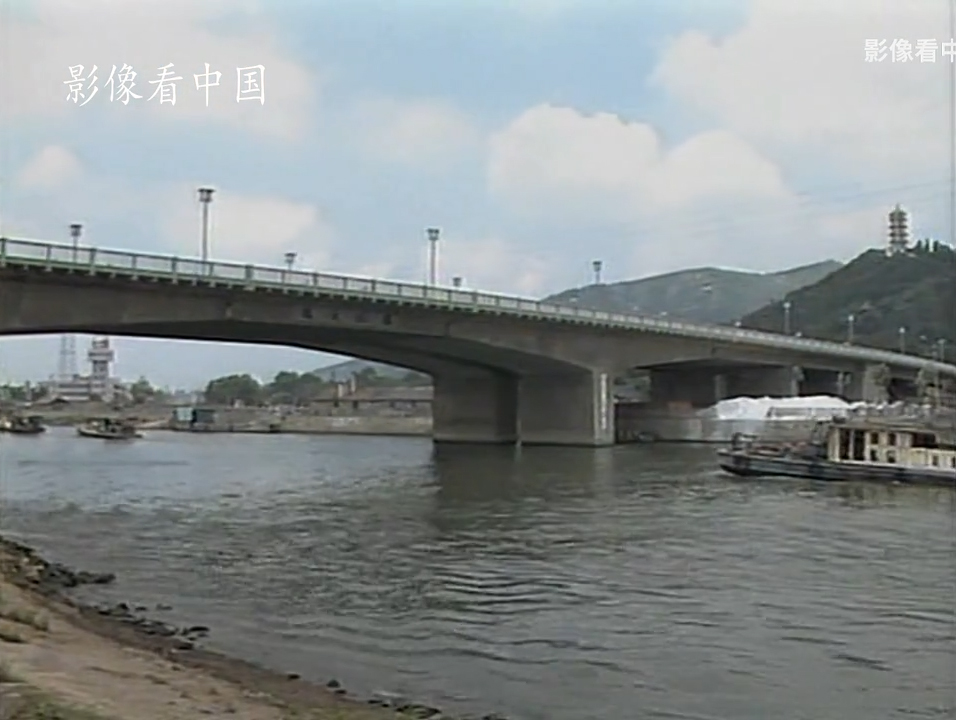
\includegraphics[width=2.5in]{img/j1.jpg}L
	\caption{Simulation results for the network.}
	\label{fig_sim}
\end{figure}


%插入latex公式
\begin{equation}
	\frac{2} {4}
	\int_a^b f(x) dx
\end{equation}



\end{document}